\documentclass[xcolor={svgnames}]{beamer}

\setbeameroption{hide notes} 

%\usetheme{NLP}
\usetheme{boxes}
\useoutertheme{infolines}

\usepackage{graphicx}
\usepackage{lmodern}
\usepackage{calc}

\usepackage{soul}

\usepackage{amsmath,amsthm,amssymb}   

\usepackage{listings}
\usepackage[style=authoryear,babel=hyphen]{biblatex}
\addbibresource{ref.bib}
\addbibresource{pliang.bib}

%\usepackage{algorithm,algorithmic}

\usepackage{tikz}
%\usepackage[debug,debugmarks]{scabby}
\usepackage{scabby}

\usepackage[customcolors]{hf-tikz}

\usepackage{mathtools}

% Text
\newcommand{\todo}[1]{\hl{\textbf{TODO:} #1}}
\newcommand{\citationneeded} {\ensuremath{^{[\textrm{citation needed}]}}}


%Math Operators
%\DeclareMathOperator {\argmax} {argmax}
%\DeclareMathOperator {\argmin} {argmin}
\DeclareMathOperator {\sgn} {sgn}
\DeclareMathOperator {\trace} {tr}
\DeclareMathOperator{\E} {\mathbb{E}}
\DeclareMathOperator{\Var} {Var}
\DeclareMathOperator{\diag} {diag}
\DeclareMathOperator{\triu} {triu}
\DeclareMathOperator{\mult} {Multinomial}
\DeclareMathOperator{\normalt} {Normal}
\DeclareMathOperator{\cvec} {cvec}

\newcommand{\ud}{\, \mathrm{d}}
\newcommand{\diff}[1] {\frac{\partial}{\, \partial #1}}
\newcommand{\difff}[2] {\frac{\partial^2}{\, \partial #1\, \partial #2}}
\newcommand{\diffn}[2] {\frac{\partial^{#2}}{\, \partial {#1}^{#2}}}
\newcommand{\tuple}[1] {\langle #1 \rangle}
\newcommand{\innerprod}[2] {\langle #1, #2 \rangle}

% Constants/etc.
\renewcommand{\Re} {\mathbb{R}}
\newcommand{\Cm} {\mathbb{C}}
\newcommand{\Qm} {\mathbb{Q}}
\newcommand{\half} {\frac{1}{2}}

\newcommand{\inv}[1] {{#1}^{-1}}

\newcommand{\normal}[2] {\mathcal{N}(#1, #2)}
\newcommand{\mL} {\mathcal{L}}

\newcommand\eqdef{\ensuremath{\stackrel{\rm def}{=}}} % Equal by definition
\newcommand\refeqn[1]{(\ref{eqn:#1})}
\newcommand\sD{\ensuremath{\mathcal{D}}}
\newcommand\sM{\ensuremath{\mathcal{M}}}
\newcommand\refapp[1]{Appendix~\ref{sec:#1}}
\newcommand\refthm[1]{Theorem~\ref{thm:#1}}
\newcommand\sigmamin{\sigma_\text{\rm min}}
\newcommand\sigmamax{\sigma_\text{\rm max}}
\newcommand\op{{\text{\rm op}}}
\newcommand\BP{\ensuremath{\mathbb{P}}}
\newcommand\reflem[1]{Lemma~\ref{lem:#1}}

%% Tensor powers
\newcommand{\tp}[1] {^{\otimes #1}}

% Matrix Perturbation
\newcommand{\pinv}[1] {#1^{\dagger}}
\newcommand{\Ap} {\hat{A}}
\newcommand{\Bp} {\hat{B}}
\newcommand{\Up} {\hat{U}}
\newcommand{\Vp} {\hat{V}}
\newcommand{\Xp} {\hat{X}}
\newcommand{\Wp} {\hat{W}}
\newcommand{\cM} {\mathcal{M}}
\newcommand{\cMp} {\hat{\mathcal{M}}}
\newcommand{\Mp} {\hat{M}}
\newcommand{\Zp} {\hat{Z}}
\newcommand{\vp} {\hat{v}}
\newcommand{\lambdap} {\hat{\lambda}}
\newcommand{\sigmap} {\hat{\sigma}}
\newcommand{\mup} {\hat{\mu}}
\newcommand{\cnd}[1] {\kappa(#1)}
\newcommand{\aerr}[1] {\varepsilon_{#1}}
\newcommand{\rerr}[1] {\delta_{#1}}
\newcommand{\serr}[1] {\alpha_{#1}}
\newcommand{\berr}[1] {\beta_{#1}}
\newcommand{\gap}[1] {\Delta_{#1}}

% Keywords
\newcommand{\Pairs}{\mathrm{Pairs}}
\newcommand{\Triples}{\mathrm{Triples}}



\newcommand<>{\drawgen}[1]{%
  \uncover#2{
    \point{start-gen}{#1}
    \node[style=node] (h) at (start-gen) {};
    \node[left=0.1cm of h] {$h$};
    \node[style=node,fill=green!70,below=1cm of h] (x) {};
    \node[left=0.1cm of x] {$x$};
    \draw[-latex] (h) -- (x);
  }
}

\newcommand<>{\drawdisc}[1]{%
  \uncover#2{
    \point{start-disc}{#1}
    \node[style=node] (h) at (start-disc) {};
    \node[right=0.1cm of h] {$h$};

    \node[style=obsnode,left=0.3cm of h] (x) {};
    \node[left=0.1cm of x] {$x$};

    \node[style=obsnode,below=1cm of h] (y) {};
    \node[left=0.1cm of y] {$y$};
    \draw[-latex] (h) -- (y);
    \draw[-latex] (x) -- (y);
  }
}

\newcommand{\tensorfactorization}[1]{%
  \point{start-tf}{#1}
  \tikzcube{tensoring}{black,fill=white}{($(start-tf) + (0,0,0)$)}{1}{1}{1};
  \node at ($(tensoring) + (1.0cm,-0.3cm)$) {$=$};
  \tensorfiber{t1}{fill=blue!70}{($(tensoring) + (2.5cm,0.0cm)$)};
  \node at ($(t1) + (1.0cm,-0.3cm)$) {$+$};
  \tensorfiber{t2}{fill=green!70}{($(t1) + (2.5cm,0.0cm)$)};
  \node at ($(t2) + (1.0cm,-0.3cm)$) {$+ \dots + $};
  \tensorfiber{t3}{fill=red!70}{($(t2) + (3.0cm,0.0cm)$)};

  \draw [decorate,decoration={brace,amplitude=10pt,raise=4pt,mirror},yshift=0pt] 
    ($(t1) + (-1cm,-1cm)$) -- ($(t3) + (0.2cm,-1cm)$) node [below,black,midway,yshift=-0.6cm] {$k$};
}

\newcommand{\matrixfactorization}[1]{%
    \point{start-mf}{#1}
    \tikzrect{mat}{black,fill=white}{($(start-mf) + (0,0)$)}{1}{1};
    \node at ($(mat) + (1.0cm,-0.3cm)$) {$=$};
    \matfiber{t1}{fill=blue!70}{($(mat) + (2.5cm,0.0cm)$)};
    \node at ($(t1) + (1.0cm,-0.3cm)$) {$+$};
    \matfiber{t2}{fill=green!70}{($(t1) + (2.5cm,0.0cm)$)};
    \node at ($(t2) + (1.0cm,-0.3cm)$) {$+ \dots + $};
    \matfiber{t3}{fill=red!70}{($(t2) + (3.0cm,0.0cm)$)};
    \draw [decorate,decoration={brace,amplitude=10pt,raise=4pt,mirror},yshift=0pt] 
      ($(t1) + (-1cm,-1cm)$) -- ($(t3) + (0.2cm,-1cm)$) node [below,black,midway,yshift=-0.6cm] {$k$};
}

\newcommand{\llhood}[2]{%
  \begin{axis}[
      x=1cm,
      y=3cm,
      scale only axis,
      height=8cm,
      width=4cm,
      axis lines*=left,
      xtick=\empty,
      ytick=\empty,
      xlabel=$\theta$,
      ylabel=$-\log p_{\theta}(x)$
      ]
    \addplot[
        black,
        thick,
        smooth,
        ] file [% Provide data as a table
          ] {data/llhood.table}
     node[pos=0.27] (em1) {}
     node[pos=0.5] (spec) {}
     node[pos=0.61] (mle) {}
     node[pos=0.85] (em2) {}
     node[pos=0.9] (em2-start) {}
     ;

  \end{axis}
}

\newcommand{\mog}[2]{%
    \begin{axis}[
        xshift=#1,
        yshift=#2,
        scale only axis,
        height=3cm,
        width=3cm,
        axis lines*=left,
        xlabel=$x_1$,
        ylabel=$x_2$,
        xtick=\empty,
        ytick=\empty,
        mark options={scale=0.2,line width=0}
        ]
      \addplot+[
          smooth,
          only marks
          ] file [% Provide data as a table
            ] {data/mog-0.table};
      \addplot+[
          smooth,
          only marks
          ] file [% Provide data as a table
            ] {data/mog-1.table};
      \addplot+[
          smooth,
          only marks
          ] file [% Provide data as a table
            ] {data/mog-2.table}
       ;

    \end{axis}
}

\newcommand{\innerpdiag}[2]{%
  \node[scale=2.0] at ($#1 + (-1.3cm,-0.3cm)$) {$\langle$};
  \node at ($#1!0.5!#2 + (-0.3cm,-0.3cm) $) {$,$};
  \node[scale=2.0] at ($#2 + (0.8cm,-0.3cm)$) {$\rangle$};
}
\newcommand{\innerpdiagv}[2]{%
  \node[scale=2.0] at ($#1 + (-0.7cm,-0.45cm)$) {$\langle$};
  \node at ($#1!0.5!#2 + (-0.1cm,-0.45cm) $) {$,$};
  \node[scale=2.0] at ($#2 + (0.4cm,-0.45cm)$) {$\rangle$};
}
\newcommand{\innerpdiagm}[2]{%
  \node[scale=2.0] at ($#1 + (-1.3cm,-0.45cm)$) {$\langle$};
  \node at ($#1!0.5!#2 + (-0.5cm,-0.45cm) $) {$,$};
  \node[scale=2.0] at ($#2 + (0.4cm,-0.45cm)$) {$\rangle$};
}
\newcommand{\innerpdiagt}[2]{%
  \node[scale=2.0] at ($#1 + (-1.3cm,-0.3cm)$) {$\langle$};
  \node at ($#1!0.5!#2 + (-0.3cm,-0.3cm) $) {$,$};
  \node[scale=2.0] at ($#2 + (0.7cm,-0.3cm)$) {$\rangle$};
}

\newcommand{\regressionA}[1]{%
    \point{start-reg-a}{#1};
    \point{start-reg-a-A}{(start-reg-a)};
    \point{start-reg-a-B}{($(start-reg-a) + (1cm,0) $)};

    \tikzrect{A}{black,fill=yellow}{($(start-reg-a-A) + (0,0)$)}{0.3}{1};
    \tikzrect{B}{black,fill=blue!70}{($(start-reg-a-B) + (0,0)$)}{0.3}{1};
    \innerpdiagv{(start-reg-a-A)}{(start-reg-a-B)};
}

\newcommand{\regressionB}[1]{%
    \point{start-reg-b}{#1};
    \point{start-reg-b-A}{(start-reg-b)};
    \point{start-reg-b-B}{($(start-reg-b) + (1.5cm,0) $)};

    \tikzrect{A}{black,fill=yellow}{($(start-reg-b-A) + (0,0)$)}{1}{1};
    \tikzrect{B}{black,fill=blue!70}{($(start-reg-b-B) + (0,0)$)}{1}{1};
    \innerpdiagm{(start-reg-b-A)}{(start-reg-b-B)};
}

\newcommand{\regressionC}[1]{%
    \point{start-reg-c}{#1};
    \point{start-reg-c-A}{(start-reg-c)};
    \point{start-reg-c-B}{($(start-reg-c) + (1.8cm,0) $)};

    \tikzcube{A}{black,fill=yellow}{($(start-reg-c-A) + (0,0)$)}{1}{1}{1};
    \tikzcube{B}{black,fill=blue!70}{($(start-reg-c-B) + (0,0)$)}{1}{1}{1};
    \innerpdiagt{(start-reg-c-A)}{(start-reg-c-B)};
}


\newcommand{\mkmlrplot}[3]{%
\begin{tikzpicture}
\begin{axis}[ 
    xshift=#1, 
    yshift=#2, 
    height=5cm, width=5cm, 
    axis lines*=left, 
    xlabel=$x$, ylabel=$y$, 
    xtick=\empty, ytick=\empty, 
    mark options={scale=0.3,line width=0},
    xmin=-1.2, xmax=1.2,
    ]
  #3
\end{axis}
\end{tikzpicture}
}


\newcommand{\mlrfull}[2]{%
  \only<1>{%
    \mkmlrplot{#1}{#2}{%
       \addplot+[blue, line width=2pt, mark=none] {0.316 + -0.862*x};
       \addplot+[green,line width=2pt, mark=none] {-0.715 + -0.268*x};
       \addplot+[red,  line width=2pt, mark=none] {-1.076 + 0.595*x};
     }
  }
  \only<2>{%
    \mkmlrplot{#1}{#2}{%
       \addplot+[blue,                 mark=none] {0.316 + -0.862*x};
       \addplot+[green,                mark=none] {-0.715 + -0.268*x};
       \addplot+[red,  line width=2pt, mark=none] {-1.076 + 0.595*x};
     }
  }
  \only<3>{%
    \mkmlrplot{#1}{#2}{%
       \addplot+[blue,                 mark=none] {0.316 + -0.862*x};
       \addplot+[green,                mark=none] {-0.715 + -0.268*x};
       \addplot+[red,  line width=2pt, mark=none] {-1.076 + 0.595*x};
       \addplot[smooth, black, only marks] table {data/mlr-1.table};
     }
  }
  \only<4>{%
    \mkmlrplot{#1}{#2}{%
       \addplot+[blue, line width=2pt, mark=none] {0.316 + -0.862*x};
       \addplot+[green,                mark=none] {-0.715 + -0.268*x};
       \addplot+[red,                  mark=none] {-1.076 + 0.595*x};
       \addplot[smooth, black, only marks] table {data/mlr-1.table};
     }
  }
  \only<5>{%
    \mkmlrplot{#1}{#2}{%
       \addplot+[blue, line width=2pt, mark=none] {0.316 + -0.862*x};
       \addplot+[green,                mark=none] {-0.715 + -0.268*x};
       \addplot+[red,                  mark=none] {-1.076 + 0.595*x};
       \addplot[smooth, black, only marks] table {data/mlr-2.table};
     }
  }
  \only<6>{%
    \mkmlrplot{#1}{#2}{%
       \addplot[smooth, black, only marks] table {data/mlr.table};
       \addplot+[blue, line width=2pt, mark=none] {0.316 + -0.862*x};
       \addplot+[green,line width=2pt, mark=none] {-0.715 + -0.268*x};
       \addplot+[red,  line width=2pt, mark=none] {-1.076 + 0.595*x};
     }
  }
  \only<7>{%
    \mkmlrplot{#1}{#2}{%
       \addplot[smooth, black, only marks] table {data/mlr.table};
     }
  }
}

\newcommand{\mlrdata}[2]{%
    \mkmlrplot{#1}{#2}{%
     \addplot[smooth, black, only marks] table {data/mlr.table};
   }
}



% these will be used later in the title page
\title[Moments and Likelihoods]{Estimating Latent Variable Graphical Models with Moments and Likelihoods}
\author[Chaganty, Liang]{%
    Arun Tejasvi Chaganty\\
    Percy Liang
}
\institute{Stanford University}

\begin{document}

% "Beamer, do the following at the start of every section"
\AtBeginSection[] 
{%
\begin{frame}<beamer> 
\frametitle{Outline} % make a frame titled "Outline"
\tableofcontents[currentsection]  % show TOC and highlight current section
\end{frame}
}

\begin{frame}
  \titlepage
\end{frame}

\section{Introduction}

\begin{frame}
  \frametitle{Latent Variable Graphical Models}

  \splitcolumn{%
      \begin{itemize}
        \item Gaussian Mixture Models \tikzmark{gmm}
        \item Latent Dirichlet Allocation
        \item Hidden Markov Models \tikzmark{hmm}
        \item PCFGs
        \item \dots
      \end{itemize}
  }{%
  \begin{canvas}
    \point{mark}{(1cm,0)};
    \point{gmm}{($(mark) + (0,+0cm)$)};
    \point{hmm}{($(mark) + (0,-1cm)$)};

    \node[anchor=south west] (mog) at (gmm) {%
      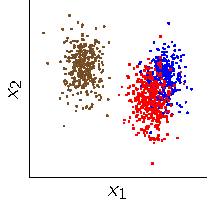
\includegraphics[width=0.45\textwidth,height=3cm,keepaspectratio]{figures/mog.pdf}
    };

    %\drawgen{($(gmm) + (0,0.0cm)$)};
    \drawhmm{(hmm)};
  \end{canvas}
  }

\end{frame}

\begin{frame}
  \frametitle{Parameter Estimation is Hard}

  \begin{tikzpicture}
    % x, y
    \llhood{0}{0};
    \node<2->[scale=0.3,circle,fill=black] at (mle) {};
    \node<2-> at ($(mle) + (0.6cm,0)$) {$\mathmb{\textrm{MLE}}$};
    \node<3->[scale=0.3,circle,fill=black] at (em1) {};
    \node<3-> at ($(em1) + (0.5cm,0)$) {$\mathmr{\textrm{EM}}$};
    \node<3->[scale=0.3,circle,fill=black] at (em2) {};
    \node<3-> at ($(em2) + (0.5cm,0)$) {$\mathmr{\textrm{EM}}$};

    \node<4->[scale=0.3,circle,fill=black] at (spec) {};
    \node<4-> at ($(spec) + (0.5cm,0.3cm)$) {$\mathmg{\textrm{MoM}}$};
   % \draw<4->[latex-latex,DarkGreen,line width=1pt] ($(mle) + (-0.8cm,0.8cm)$) -- node[above]{$\mathmg{\epsilon}$} ($(mle) + (+0.8cm,0.8cm)$);
  \end{tikzpicture}

  % Simple message: MLE is consistent but intractable, EM is efficient not but consistent. Can we get something in between.

  \begin{itemize}
    \item<1-> Log-likelihood function is non-convex.
    \item<2-> MLE is consistent but intractable.
    \item<3-> Local methods (EM, gradient descent, etc.) are tractable but inconsistent\alt<3-4>{.}{\em~and generalize easily.}
    \item<4-> {\em Method of moments} estimators can be consistent and
      computationally-efficient, but more data. 
         \uncover<6->{\bf Thus far, applicable to a limited set of models.}
  \end{itemize}
\end{frame}

\begin{frame}
  \frametitle{Main contributions}

  \splitcolumn{%
    \begin{itemize}
     % \item {\em Before our work}
     % \begin{itemize}
     %   \item Gaussian Mixture Models \tikzmark{gmm}
     %   \item Hidden Markov Models 
     %   \item Latent Dirichlet Allocation
     % \end{itemize}
     \item<2-> An algorithm for a {\bf broader model family} with
       succinct conditions. \tikzmark{grid}
    \item<3-> Efficiently learn models with low-degree but {\bf high-treewidth}.
    \item<3-> Extends to {\bf log-linear models}.
    \item<4-> Combine moment estimators with composite
      likelihood estimators.
    \end{itemize}
  }{%
  \begin{canvas}
    \point{mark}{(4cm,0)};
    %\point{gmm}{({pic cs:gmm} -| mark)};
    %\point{grid}{({pic cs:grid} -| mark)};
    \point{gmm}{($(mark) + (0,3cm)$)};
    \point{grid}{($(mark) + (0,-1cm)$)};

%    \node[anchor=south west] (mog) at (gmm) {%
%      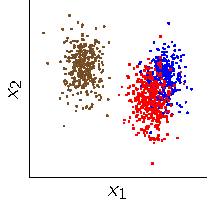
\includegraphics[width=0.45\textwidth,height=3cm,keepaspectratio]{figures/mog.pdf}
%    };

    \drawgen{($(gmm) + (0,0.0cm)$)};
    \drawgrid<2->{(grid)};
  \end{canvas}
  }


%  \cornertext<1->{\cite{AnandkumarGeHsu2012}}
%
%  \begin{canvas}
%    % Tasks.
%
%    \node<1->[anchor=west] (diag) at (-3cm, 1cm) {%
%      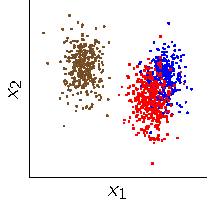
\includegraphics[width=0.45\textwidth,height=3cm,keepaspectratio]{figures/mog.pdf}
%    };
%    %\drawgen{(-3cm,1cm)}
%    \node[below=0.6cm of diag.south] {Before};
%
%    % Highlight
%    \draw<2>[scale=0.8,fill=green,opacity=0.4,dashed] (1cm,2.5cm) rectangle (6.5cm,-2.5cm);
%      \drawgrid{(3cm,1cm)}
%      \node[below=0.1cm of h4.south] {After};
%  \end{canvas}

\end{frame}

% \begin{frame}
%   \frametitle{Related Work}
%   \begin{itemize}
%     \item<1-> Method of Moments [Pearson, 1894]
%     \item<2-> Observable operators
%     \begin{itemize}
%       \item Control Theory [Ljung, 1987]
%       \item Observable operator models [Jaeger, 2000; {\small{Littman/Sutton/Singh, 2004}}]
%       \item Hidden Markov models [Hsu/Kakade/Zhang, 2009]
%       \item Low-treewidth graphs [Parikh et al., 2012]
%       \item Weighted finite state automata [Balle \& Mohri, 2012]
%     \end{itemize}
%      \item<3-> Parameter Estimation
%   \begin{itemize}
%     \item Mixture of Gaussians [Kalai/Moitra/Valiant, 2010]
%     \item \alert{Mixture models, HMMs [Anandkumar/Hsu/Kakade, 2012]}
%     \item Latent Dirichlet Allocation [Anandkumar/Hsu/Kakade, 2012]
%     \item Stochastic block models [Anandkumar/Ge/Hsu/Kakade, 2012]
%     \item Linear Bayesian networks [Anandkumar/Hsu/Javanmard/Kakade, 2012]
%   \end{itemize}
%   \end{itemize}
% \end{frame}

\section{Three-view Mixture Models}

\begin{frame}
  \frametitle{Three-view Mixture Models}
  \cornertext<1->{\cite{AnandkumarGeHsu2012}}
  \begin{canvas}
    % The model
    \point{mark}{(1cm,0)};
    \point{start}{(1cm,1cm)}; %{pic cs:gen} -| mark)};
    \drawgen<1->{($(start) + (-4cm,1cm)$)};
    %\node[anchor=west] (diag1) at ($(start)$) {%
    %  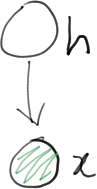
\includegraphics[width=0.45\textwidth,height=2cm,keepaspectratio]{figures/gen.png}
    %};
    \node<1->[anchor=west] (diag) at ($(start) + (0cm,0.0cm)$) {%
      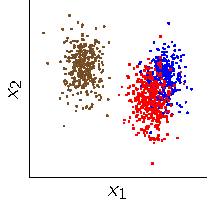
\includegraphics[width=0.45\textwidth,height=3cm,keepaspectratio]{figures/mog.pdf}
    };

    \node<6-> (bottleneck) at ($(x2.south) - (0,0.4cm)$) {\textmb{\bf Bottleneck}};

    \uncover<2>{
    \vectorfactorization{(-3cm,-2cm)}
    }
    \uncover<3>{
    \matrixfactorization{(-3cm,-2cm)}
    }


    \node<5-> (tf) at ($(t3.north) + (-1cm,0.5cm)$) {Tensor eigen-decomposition};

    \uncover<4->{
    \tensorfactorization{(-3cm,-2cm)}
    }

  \end{canvas}
\end{frame}

\begin{frame}
  \frametitle{}

  \begin{canvas}
    % Tasks.
    \drawgen{(-3cm,1cm)}
    \node[below=0.1cm of x2.south] {Bottlenecked};

    % Highlight
    \draw<2>[scale=0.8,fill=green,opacity=0.4,dashed] (1cm,3.0cm) rectangle (6.5cm,-3.0cm);
      \drawgrid{(3cm,1cm)}
      \node[below=0.8cm of h4.south] {Uniformly bottlenecked};

  \end{canvas}

\end{frame}

\section{Uniformly Bottlenecked Models}

\begin{frame}
  \frametitle{Example: a grid model.}
  \splitcolumn{%
    \begin{itemize}
      \item<2-> Bottleneck! $\Pr(x_i^a | h_i)$.
      \item<4-> Linear relation! $\Pr(x_1^b) = \Pr(x_1^b | h_1) \mathmg{\Pr(h_1)}$.
      \item<6-> Linear relation! $\Pr(x_1^b, x_3^a) = \Pr(x_1^b | h_1) \Pr(x_3^b | h_3) \Pr(h_1) \mathmg{\Pr(h_3 | h_1)}$.
      \item<8-> Linear relation! $\Pr(x_2^b, x_3^b, x_4^b) = \Pr(x_2^b | h_2) \Pr(x_3^b | h_3) \Pr(x_4^b | h_4)$\\
        $\mathmg{\Pr(h_4 | h_2, h_3)} \Pr(h_2) \Pr(h_3)$.
      \item<10-> {\bf Solving the bottlenecks has made the problem easy!}
    \end{itemize}
  }{%
  \begin{canvas}
    \point{mark}{(3cm,0)};
    \point{start-grid}{(mark)};
   \node[style=node, scale=0.8] (h1) at (start-grid) {$h_1$};
   \node[style=node, scale=0.8, below left= 0.5cm of h1] (h2) {$h_2$};
   \node[style=node, scale=0.8, below right= 0.5cm of h1] (h3) {$h_3$};
   \node[style=node, scale=0.8, below right= 0.5cm of h2] (h4) {$h_4$};

   \point{pi}{($(h1.north) + (0,0.1cm)$)};
   \draw[-latex] (h1) -- node[scale=0.7,above] (T1) {} (h2);
   \draw[-latex] (h1) -- node[scale=0.7,above] (T2) {} (h3);
   \draw[-latex] (h2) -- (h4);
   \draw[-latex] (h3) -- (h4);
   \point{V}{($(h4.north) + (0,0.1cm)$)};

% Observed nodes
   \node[style=obsnode, scale=0.7, above left=0.3cm of h1] (x1a) {$x^a_1$};
   \node[style=obsnode, scale=0.7, above right=0.3cm of h1] (x1b) {$x^b_1$};
   \draw[-latex] (h1) -- (x1a);
   \draw[-latex] (h1) -- (x1b);

   \node[style=obsnode, scale=0.7, above left=0.3cm of h2] (x2a) {$x^a_2$};
   \node[style=obsnode, scale=0.7, below left=0.3cm of h2] (x2b) {$x^b_2$};
   \draw[-latex] (h2) -- node[scale=0.7,above] (O1) {} (x2a);
   \draw[-latex] (h2) -- node[scale=0.7,below] (O2) {} (x2b);

   \node[style=obsnode, scale=0.7, above right=0.3cm of h3] (x3a) {$x^a_3$};
   \node[style=obsnode, scale=0.7, below right=0.3cm of h3] (x3b) {$x^b_3$};
   \draw[-latex] (h3) -- (x3a);
   \draw[-latex] (h3) -- (x3b);
    
   \node[style=obsnode, scale=0.7, below left=0.3cm of  h4] (x4a) {$x^a_4$};
   \node[style=obsnode, scale=0.7, below right=0.3cm of h4] (x4b) {$x^b_4$};

   \draw[-latex] (h4) -- (x4a);
   \draw[-latex] (h4) -- (x4b);

   % Story - 
  \begin{pgfonlayer}{background}
  \draw<2>[draw=black,fill=green!70,rounded corners,line width=1pt, dotted] 
                  ($(x2a.north west) + (135:0.3cm)$) -- 
                  ($(x2b.south west) + (-135:0.3cm)$) -- 
                  ($(x4a.south east) + (-45:0.3cm)$) -- 
                  ($(h2.east) + (0:0.3cm)$) -- 
                  ($(x2a.north east) + (45:0.3cm)$) -- 
                  cycle;
  \draw<4>[draw=black,fill=green!70,rounded corners,line width=1pt, dotted] 
                  ($(x1a.north west) + (135:0.3cm)$) -- 
                  ($(x1a.north east) + (45:0.3cm)$) -- 
                  ($(h1.south east) + (-45:0.3cm)$) -- 
                  ($(h1.south west) + (-135:0.3cm)$) -- 
                  cycle;
  \draw<6>[draw=black,fill=green!70,rounded corners,line width=1pt, dotted] 
                  ($(x1b.north west) + (135:0.3cm)$) -- 
                  ($(x3a.north east) + (45:0.3cm)$) -- 
                  ($(h3.south east) + (-45:0.3cm)$) -- 
                  ($(h1.south west) + (-135:0.3cm)$) -- 
                  cycle;
  \draw<8>[draw=black,fill=green!70,rounded corners,line width=1pt, dotted] 
                  ($(h2.north west) + (135:0.3cm)$) -- 
                  ($(x2b.south west) + (-135:0.3cm)$) -- 
                  ($(x4a.south west) + (-135:0.3cm)$) -- 
                  ($(x4b.south east) + (-45:0.3cm)$) -- 
                  ($(x3b.north east) + (45:0.3cm)$) -- 
                  ($(h3.north east) + (45:0.3cm)$) -- 
                  cycle;
  \end{pgfonlayer}

   \node<1>[scale=1.0] at (pi) {$\mathmg{\pi}$};
   \node<1>[scale=1.0] at (T1) {$\mathmg{T}$};
   \node<1>[scale=1.0] at (T2) {$\mathmg{T}$};
   \node<1>[scale=1.0] at (V) {$\mathmg{V}$};
   \node<1>[scale=1.0] at (O1) {$\mathmg{O}$};
   \node<1>[scale=1.0] at (O2) {$\mathmg{O}$};

   \node<3->[scale=1.0] at (O1) {\textmg{\checkmark}};
   \node<3->[scale=1.0] at (O2) {\textmg{\checkmark}};

   \node<5->[scale=1.0] at (pi) {\textmg{\checkmark}};

   \node<7->[scale=1.0] at (T1) {\textmg{\checkmark}};
   \node<7->[scale=1.0] at (T2) {\textmg{\checkmark}};

   \node<9->[scale=1.0] at (V) {\textmg{\checkmark}};

  \end{canvas}
  }
\end{frame}
\begin{frame}
  \frametitle{Views and Bottlenecks}
  \begin{itemize}
    \item<+-> {\bf Key insight:} Easy to learn latent parameters given a view $\Pr(x|h)$. 
    \item<+-> For any clique, if each hidden variable has a unique
      view, the distribution of the hidden variables is just a linear equation!
    \item<+-> {\bf Uniformly bottlenecked}: Every hidden variable has
      atleast three conditionally independent observed variables.
      \sidenote{Guarantees unique views.}
    \item<+-> Algorithm: (a) estimate $\Pr(x|h)$ using bottlenecks, (b)
      solve a linear equation between $\Pr(h_1,\cdots,h_m)$ and $P(x_1,
      \cdots, x_m)$.
    \item<+-> {\bf Assumptions}: For every clique $\Pr(h_1, \cdots, h_m)$,
      every conditioning $\Pr(h_1, \cdots, h_k | h_{k+1}, \cdots h_m)$
      is ``full-rank''.
  \end{itemize}
  
\end{frame}
\begin{frame}
  \frametitle{More Uniformly Bottlenecked Examples}
  \begin{canvas}
    \drawhmm<1->{(-4cm, 2cm)};
    \node at ($(start-hmm) + (0, 0.6cm)$) {Hidden Markov models};
    \drawtree<1->{(2cm, 2cm)};
    \node at ($(start-tree) + (0, 0.6cm)$) {Latent Tree models};
    \drawnoisyor<3->{(0cm, -2cm)};
    \node<3-> at ($(start-nor) + (0, 0.7cm)$) {Noisy Or (non-example)};

% \begin{pgfonlayer}{background}
% \draw<2->[rounded corners,line width=1pt, dotted, black] 
%                 ($(h2.north east) + (45:0.2cm)$) -- 
%                 ($(x3.north east) + (45:0.2cm)$) -- 
%                 ($(x3.south east) + (-45:0.2cm)$) -- 
%                 ($(x1.south west) + (-135:0.2cm)$) -- 
%                 ($(x1.north west) + (135:0.2cm)$) -- 
%                 ($(h2.north west) + (135:0.2cm)$) -- 
%                 cycle;
% \end{pgfonlayer}
% 
% \begin{pgfonlayer}{background}
% \draw<2>[rounded corners,line width=1pt, dotted, black] 
%                 ($(h4.north east) + (45:0.2cm)$) -- 
%                 ($(x4b.north east) + (45:0.2cm)$) -- 
%                 ($(x4b.south east) + (-45:0.2cm)$) -- 
%                 ($(x3b.south west) + (-135:0.2cm)$) -- 
%                 ($(x3b.north west) + (135:0.2cm)$) -- 
%                 ($(h4.north west) + (135:0.2cm)$) -- 
%                 cycle;
% \end{pgfonlayer}


  \end{canvas}

\end{frame}

% Efficiency 1: EM (+diagram).
\section{Combining with likelihood estimators}
\begin{frame}
  \frametitle{Convex composite likelihoods}
  \splitcolumn{%
    \begin{itemize}
      \item<1-> Given the observed marginals, $\Pr(x|h)$, the hidden marginals
        $\Pr(h_1, \cdots, h_m)$ is linearly related.
      \item<2-> The composite log-likelihood over $x_1, \cdots, x_m$ is
        actually convex!
      \item<3-> Running EM will converge and is more statistically efficient.
    \end{itemize}
  }{%
    \begin{canvas}
      \point{stuff}{(3cm,0cm)};
      \node<1>[scale=0.5] at (0.5cm,0) {\llhood{3.5}{0}};
      \node<2->[anchor=center] (obj) at (stuff) {%
      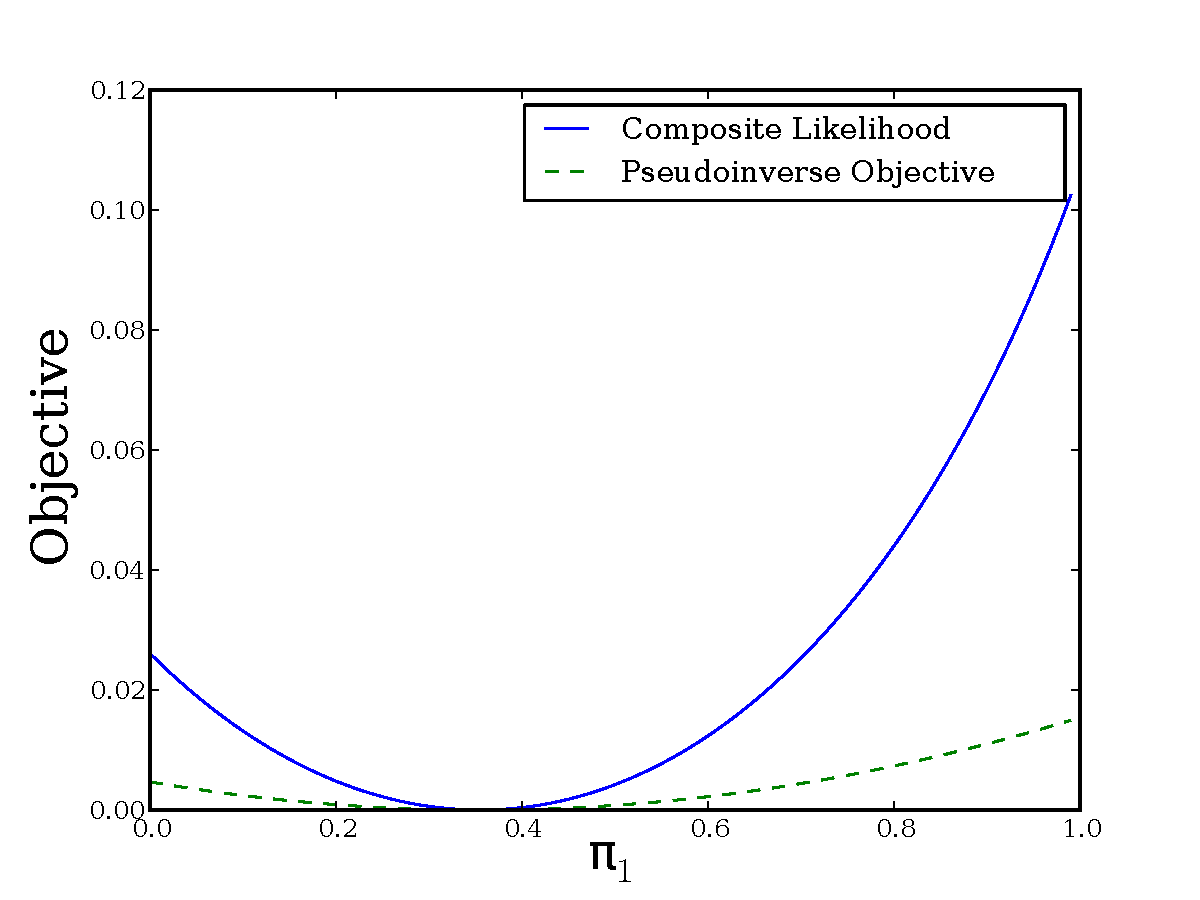
\includegraphics[width=\textwidth,height=6cm,keepaspectratio]{figures/piecewise-objective.pdf}
      };
    \end{canvas}
  }
\end{frame}

\section{Log-linear models}
\begin{frame}
  \frametitle{Log-linear models}
  \begin{itemize}
    \item<1-> $p_\theta(\bx, \bh) = \exp\left( \theta^\top \phi(\bx,\bh) - A(\theta) \right)$.
    \item<2-> The {\em unsupervised} negative log-likelihood is non-convex,
        \begin{align*}
        L_\text{unsup}(\theta) \eqdef \E_{\bx \sim \sD}[\log \sum_{\bh \in \sH} p_\theta(\bx,\bh)].
        \end{align*}
  \end{itemize}
\end{frame}

\begin{frame}
  \frametitle{Estimation is convex with marginals}
  \begin{itemize}
    \item<1-> $p_\theta(\bx, \bh) = \exp\left( \theta^\top \phi(\bx,\bh) - A(\theta) \right)$.
      \item<1-> In the supervised case with $\bh$ though, the objective {\em is convex},
        \begin{align*}
        \label{eqn:logLinearSupervised}
        L_\text{sup}(\theta) &\eqdef \E_{(\bx,\bh) \sim \sD_\text{sup}}[\log p_\theta(\bx,\bh)] \\
                             &= \theta^\top \left(\sum_{\sC \in \sG} \E[\phi(\bx_\sC,\bh_\sC)]\right) - A(\theta).
        \end{align*}
      \item<2-> {\bf Key idea:} We can estimate marginals $\E_{(\bx,\bh) \sim \sD_\text{sup}}[\log p_\theta(\bx,\bh)]$!
  \end{itemize}
\end{frame}

\section{Conclusions}

\begin{frame}
  \frametitle{Conclusions}
  \begin{itemize}
      \item Uniformly bottlenecked models
      \item Scales with the size of each clique, not the tree-width
      \item Solving bottlenecks breaks problem into convex pieces; can be solved more accurately
      \item The marginals make the log-linear recovery problem convex.
  \end{itemize}
\end{frame}

\begin{frame}
  \frametitle{}
    Thank you!
\end{frame}

\end{document}

